%% LyX 1.1 created this file.  For more info, see http://www.lyx.org/.
%% Do not edit unless you really know what you are doing.
\documentclass[english]{article}
\usepackage[OT1]{fontenc}
\usepackage[latin1]{inputenc}
\usepackage{geometry}
\geometry{verbose,letterpaper,tmargin=1in,bmargin=1in,lmargin=1in,rmargin=1in}
\usepackage{babel}
\usepackage{graphics}
\usepackage{verbatim}
\usepackage{subfigure}

\makeatletter

%%%%%%%%%%%%%%%%%%%%%%%%%%%%%% LyX specific LaTeX commands.
\providecommand{\LyX}{L\kern-.1667em\lower.25em\hbox{Y}\kern-.125emX\@}

\makeatother
\begin{document}

\section{Introduction}

SciPy is a collection of mathematical algorithms and convenience functions
built on the Numeric extension for Python. It adds significant power
to the interactive Python session by exposing the user to high-level
commands and classes for the manipulation and visualization of data.
With SciPy, an interactive Python session becomes a data-processing
and system-prototyping environment rivaling sytems such as Matlab,
IDL, Octave, R-Lab, and SciLab. 

The additional power of using SciPy within Python, however, is that
a powerful programming language is also available for use in developing
sophisticated programs and specialized applications. Scientific applications
written in SciPy benefit from the development of additional modules
in numerous niche's of the software landscape by developers across
the world. Everything from parallel programming to web and data-base
subroutines and classes have been made available to the Python programmer.
All of this power is available in addition to the mathematical libraries
in SciPy.

This document provides a tutorial for the first-time user of SciPy
to help get started with some of the features available in this powerful
package. It is assumed that the user has already installed the package.
Some general Python facility is also assumed such as could be acquired
by working through the Tutorial in the Python distribution. Throughout
this tutorial it is assumed that the user has imported all of the
names defined in the SciPy namespace using the command \begin{verbatim}
>>> from scipy import *\end{verbatim} 


\section{General help}

Python provides the facility of documentation strings. The functions
and classes available in SciPy use this method for on-line documentation.
There are two methods for reading these messages and getting help.
Python provides the command \textbf{help} in the pydoc module. Entering
this command with no arguments (i.e. \textgreater{}\textgreater{}\textgreater{}
help ) launches an interactive help session that allows searching
through the keywords and modules available to all of Python. Running
the command help with an object as the argument displays the calling
signature, and the documentation string of the object.

The pydoc method of help is sophisticated but uses a pager to display
the text. Sometimes this can interfere with the terminal you are running
the interactive session within. A scipy-specific help system is also
available under the command scipy.help. The signature and documntation
string for the object passed to the help command are printed to standard
output (or to a writeable object passed as the third argument). The
second keyword argument of {}``scipy.help{}'' defines the maximum
width of the line for printing.

If a module is passed as the argument to help than a list of the functions
and classes defined in that module is printed. For example:

\verbatiminput{example2.1}


\section{Special Functions (special)}


\subsection{Vectorizing functions (special.general\_function)}

One of the features that the \textbf{special} sub-package provides
is a class \textbf{general\_function} to convert an ordinary Python
function which accepts scalars and returns scalars into a {}``vectorized-function{}''
with the same broadcasting rules as other Numeric functions (\emph{i.e.}
the Universal functions, or ufuncs). For example, suppose you have
a Python function named \textbf{addsubtract} defined as:

\verbatiminput{example3.1}which defines a function of two scalar
variables and returns a scalar result. The class general\_function
can be used to {}``vectorize{}'' this function so that \begin{verbatim}
>>> vec_addsubstract = special.general_function(addsubtract) \end{verbatim} 
\noindent returns a function which takes array arguments and returns
an array result:

\verbatiminput{example3.2}


\subsection{Special Functions}

The main feature of the \textbf{special} package is the definition
of numerous special functions of mathematical physics. Available are
airy, elliptic, bessel, gamma, beta, hypergeometric, and several statistical
functions. All of these functions behave can take array arguments
and return array results following the same broadcasting rules as
other math functions in Numerical Python. For a complete list of these
functions with a one-line description type \texttt{>>>help(special).}
Each function also has it's own documentation accessible using help.


\section{Integration (integrate)}

The \textbf{integrate} sub-package provides several integration techniques
including an ordinary differential equation integrator. An overview
of the module is provided by the help command:

\verbatiminput{example4.1}


\subsection{General integration (integrate.quad)}

The function \textbf{quad} is provided to integrate a function of
one variable between two points. The points can be \( \pm \infty  \)
(\( \pm  \)\textbf{integrate.inf}) to indicate infinite limits. For
example, suppose you wish to integrate a bessel function \texttt{jv(2.5,x)}
along the interval \( [0,4.5]. \) \[
I=\int _{0}^{4.5}J_{2.5}\left( x\right) \, dx.\]
 This could be computed using \textbf{quad:}

\verbatiminput{example4.2}

The first argument to quad is a {}``callable{}'' Python object (\emph{i.e}
a function, method, or class instance). Notice the use of a lambda-function
in this case as the argument. The next two arguments are the limits
of integration. The return value is a tuple, with the first element
holding the estimated value of the integral and the second element
holding an upper bound on the error. Notice, that in this case, the
true value of this integral is \[
I=\sqrt{\frac{2}{\pi }}\left( \frac{18}{27}\sqrt{2}\cos \left( 4.5\right) -\frac{4}{27}\sqrt{2}\sin \left( 4.5\right) +\sqrt{2\pi }\textrm{Si}\left( \frac{3}{\sqrt{\pi }}\right) \right) ,\]
 where \[
\textrm{Si}\left( x\right) =\int _{0}^{x}\sin \left( \frac{\pi }{2}t^{2}\right) \, dt.\]
 is the Fresnel sine integral. Note that the numerically-computed
integral is within \( 1.04\times 10^{-11} \) of the exact result
--- well below the reported error bound. 

Infinite inputs are also allowed in \textbf{quad} by using \( \pm  \)\textbf{integrate.inf}
as one of the arguments. For example, suppose that a numerical value
for the exponential integral:\[
E_{n}\left( x\right) =\int _{1}^{\infty }\frac{e^{-xt}}{t^{n}}\, dt.\]
 is desired (and the fact that this integral can be computed as \texttt{special.expn(n,x)}
is forgotten). The functionality of the function \textbf{special.expn}
can be replicated by defining a new function \textbf{vec\_expint}
based on the routine \textbf{quad: }

\verbatiminput{example4.3} 

The function which is integrated can even use the quad argument (though
the error bound may underestimate the error due to possible numerical
error in the integrand from the use of \textbf{quad}). The integral
in this case is \[
I_{n}=\int _{0}^{\infty }\int _{1}^{\infty }\frac{e^{-xt}}{t^{n}}\, dt\, dx=\frac{1}{n}.\]


\verbatiminput{example4.4}

This last example shows that multiple integration can be handled using
repeated calls to \textbf{quad.} The mechanics of this for double
and triple integration have been wrapped up into the functions \textbf{dblquad}
and \textbf{tplquad.} The function, \textbf{dblquad} performs double
integration. Use the help function to be sure that the arguments are
defined in the correct order. In addition, the limits on all inner
integrals are actually functions which can be constant functions.
An example of using double integration to compute several values of
\( I_{n} \) is shown below:

\verbatiminput{example4.5}


\subsection{Ordinary differential equations (integrate.odeint)}

Integrating a set of ordinary differential equations (ODEs) given
initial conditions is another useful example. The function \textbf{odeint}
is available in SciPy for integrating a first-order vector differential
equation:\[
\frac{d\mathbf{y}}{dt}=\mathbf{f}\left( \mathbf{y},t\right) ,\]
 given initial conditions \( \mathbf{y}\left( 0\right) =y_{0}, \)
where \( \mathbf{y} \) is a length \( N \) vector and \( \mathbf{f} \)
is a mapping from \( {\cal R}^{N} \) to \( {\cal R}^{N}. \) A higher-order
ordinary differential equation can always be reduced to a differential
equation of this type by introducing intermediate derivatives into
the \( \mathbf{y} \) vector. 

For example suppose it is desired to find the solution to the following
second-order differential equation:\[
\frac{d^{2}w}{dz^{2}}-zw(z)=0\]
 with initial conditions \( w\left( 0\right) =\frac{1}{\sqrt[3]{3^{2}}\Gamma \left( \frac{2}{3}\right) } \)
and \( \left. \frac{dw}{dz}\right| _{z=0}=-\frac{1}{\sqrt[3]{3}\Gamma \left( \frac{1}{3}\right) }. \)
It is known that the solution to this differential equation with these
boundary conditions is the Airy function \[
w=\textrm{Ai}\left( z\right) ,\]
 which gives a means to check the integrator using \textbf{special.airy. }

First, convert this ODE into standard form by setting \( \mathbf{y}=\left[ \frac{dw}{dz},w\right]  \)
and \( t=z. \) Thus, the differential equation becomes\[
\frac{d\mathbf{y}}{dt}=\left[ \begin{array}{c}
ty_{1}\\
y_{0}
\end{array}\right] =\left[ \begin{array}{cc}
0 & t\\
1 & 0
\end{array}\right] \left[ \begin{array}{c}
y_{0}\\
y_{1}
\end{array}\right] =\left[ \begin{array}{cc}
0 & t\\
1 & 0
\end{array}\right] \mathbf{y}.\]
 In other words, \[
\mathbf{f}\left( \mathbf{y},t\right) =\mathbf{A}\left( t\right) \mathbf{y}.\]
 

As an interesting reminder, if \( \mathbf{A}\left( t\right)  \) commutes
with \( \int _{0}^{t}\mathbf{A}\left( \tau \right) \, d\tau  \) under
matrix multiplication, then this linear differential equation has
an exact solution using the matrix exponential: \[
\mathbf{y}\left( t\right) =\exp \left( \int _{0}^{t}\mathbf{A}\left( \tau \right) d\tau \right) \mathbf{y}\left( 0\right) ,\]
 However, in this case, \( \mathbf{A}\left( t\right)  \) and its
integral do not commute.

There are many optional inputs and outputs available when using odeint
which can help tune the solver. These additional inputs and outputs
are not needed much of the time, however, and the three required input
arguments and the output solution suffice. The required inputs are
the function defining the derivative, \emph{fprime,} the initial conditions
vector, \emph{y0}, and the time points to obtain a solution, \emph{t,}
(with the initial value point as the first element of this sequence).
The output to \textbf{odeint} is a matrix where each row contains
the solution vector at each requested time point (thus, the initial
conditions are given in the first output row). 

The following example illustrates the use of odeint including the
usage of the \textbf{Dfun} option which allows the user to specify
a gradient (with respect to \( \mathbf{y} \)) of the function, \textbf{\( \mathbf{f}\left( \mathbf{y},t\right)  \).}

\verbatiminput{example4.6}


\subsection{Gaussian quadrature (integrate.gauss\_quadtol)}

A few functions are also provided in order to perform simple Gaussian
quadrature over a fixed interval. The first is \textbf{gauss\_quad}
which performs fixed-order Gaussian quadrature. The second function
is \textbf{gauss\_quadtol} which performs Gaussian quadrature of multiple
orders until the difference in the integral estimate is beneath some
tolerance supplied by the user. These functions both use the module
\textbf{integrate.orthogonal} which can calculate the roots and quadrature
weights of a large variety of orthogonal polynomials.


\section{Optimization (optimize)}

There are several classical optimization algorithms provided by SciPy
in the \textbf{optimize} package. An overview of the module is available
using \textbf{help} (or pydoc.help):

\verbatiminput{example5.1} The first four algorithms are unconstrained
minimization algorithms (fmin: Nelder-Mead simplex, fmin\_bfgs: BFGS,
fmin\_ncg: Newton Conjugate Gradient, and leastsq: Levenburg-Marquardt).
The fourth algorithm only works for functions of a single variable
but allows minimization over a specified interval. The last algorithm
actually finds the roots of a general function of possibly many variables.
It is included in the optimization package because at the (non-boundary)
extreme points of a function, the gradient is equal to zero.


\subsection{Nelder-Mead Simplex algorithm (optimize.fmin)}

The simplex algorithm is probably the simplest way to minimize a fairly
well-behaved function. The simplex algorithm requires only function
evaluations and is a good choice for simple minimization problems.
However, because it does not use any gradient evaluations, it may
take longer to find the minimum. To demonstrate the minimization function
consider the problem of minimizing the Rosenbrock function of \( N \)
variables:\[
f\left( \mathbf{x}\right) =\sum _{i=1}^{N-1}100\left( x_{i}-x_{i-1}^{2}\right) ^{2}+\left( 1-x_{i-1}\right) ^{2}.\]
 The minimum value of this function is 0 which is achieved when \( x_{i}=1. \)
This minimum can be found using the \textbf{fmin} routine as shown
in the example below:

\verbatiminput{example5.2}


\subsection{Broyden-Fletcher-Goldfarb-Shanno algorithm (optimize.fmin\_bfgs)}

In order to converge more quickly to the solution, this routine uses
the gradient of the objective function. If the gradient is not given
by the user, then it is estimated using first-differences. The Broyden-Fletcher-Goldfarb-Shanno
(BFGS) method requires fewer function calls than the simplex algorithm
but unless the gradient is provided by the user, the speed savings
won't be significant.

To demonstrate this algorithm, the Rosenbrock function is again used.
The gradient of the Rosenbrock function is the vector: \begin{eqnarray*}
\frac{\partial f}{\partial x_{j}} & = & \sum _{i=1}^{N}200\left( x_{i}-x_{i-1}^{2}\right) \left( \delta _{i,j}-2x_{i-1}\delta _{i-1,j}\right) -2\left( 1-x_{i-1}\right) \delta _{i-1,j}.\\
 & = & 200\left( x_{j}-x^{2}_{j-1}\right) -400x_{j}\left( x_{j+1}-x_{j}^{2}\right) -2\left( 1-x_{j}\right) .
\end{eqnarray*}
This expression is valid for the interior derivatives. Special cases
are\begin{eqnarray*}
\frac{\partial f}{\partial x_{0}} & = & -400x_{0}\left( x_{1}-x_{0}^{2}\right) -2\left( 1-x_{0}\right) ,\\
\frac{\partial f}{\partial x_{N-1}} & = & 200\left( x_{N-1}-x_{N-2}^{2}\right) .
\end{eqnarray*}
 A Python function which computes this gradient is constructed by
the code-segment:

\verbatiminput{example5.3}

The calling signature for the BFGS minimization algorithm is similar
to \textbf{fmin} with the addition of the \emph{fprime} argument.
An example usage of \textbf{fmin\_bfgs} is shown in the following
example which minimizes the Rosenbrock function.

\verbatiminput{example5.4}


\subsection{Newton-Conjugate-Gradient (optimize.fmin\_ncg)}

The method which requires the fewest function calls and is therefore
often the fastest method to minimize functions of many variables is
\textbf{fmin\_ncg.} This method is a modified Newton's method and
uses a conjugate gradient algorithm to (approximately) invert the
local Hessian. Newton's method is based on fitting the function locally
to a quadratic form:\[
f\left( \mathbf{x}\right) \approx f\left( \mathbf{x}_{0}\right) +\nabla f\left( \mathbf{x}_{0}\right) \cdot \left( \mathbf{x}-\mathbf{x}_{0}\right) +\frac{1}{2}\left( \mathbf{x}-\mathbf{x}_{0}\right) ^{T}\mathbf{H}\left( \mathbf{x}_{0}\right) \left( \mathbf{x}-\mathbf{x}_{0}\right) .\]
 where \( \mathbf{H}\left( \mathbf{x}_{0}\right)  \) is a matrix
of second-derivatives (the Hessian). If the Hessian is positive definite
then the local minimum of this function can be found by setting the
gradient of the quadratic form to zero, resulting in \[
\mathbf{x}_{\textrm{opt}}=\mathbf{x}_{0}-\mathbf{H}^{-1}\nabla f.\]
 The inverse of the Hessian is evaluted using the conjugate-gradient
method. An example of employing this method to minimizing the Rosenbrock
function is given below. To take full advantage of the NewtonCG method,
a function which computes the Hessian must be provided. The Hessian
matrix itself does not need to be constructed, only a vector which
is the product of the Hessian with an arbitrary vector needs to be
available to the minimization routine. As a result, the user can provide
either a function to compute the Hessian matrix, or a function to
compute the product of the Hessian with an arbitrary vector. 


\subsubsection{Full Hessian example:}

The Hessian of the Rosenbrock function is \begin{eqnarray*}
H_{ij}=\frac{\partial ^{2}f}{\partial x_{i}\partial x_{j}} & = & 200\left( \delta _{i,j}-2x_{i-1}\delta _{i-1,j}\right) -400x_{i}\left( \delta _{i+1,j}-2x_{i}\delta _{i,j}\right) -400\delta _{i,j}\left( x_{i+1}-x_{i}^{2}\right) +2\delta _{i,j},\\
 & = & \left( 202+1200x_{i}^{2}-400x_{i+1}\right) \delta _{i,j}-400x_{i}\delta _{i+1,j}-400x_{i-1}\delta _{i-1,j},
\end{eqnarray*}
 if \( i,j\in \left[ 1,N-2\right]  \) with \( i,j\in \left[ 0,N-1\right]  \)
defining the \( N\times N \) matrix. Other non-zero entries of the
matrix are \begin{eqnarray*}
\frac{\partial ^{2}f}{\partial x_{0}^{2}} & = & 1200x_{0}^{2}-400x_{1}+2,\\
\frac{\partial ^{2}f}{\partial x_{0}\partial x_{1}}=\frac{\partial ^{2}f}{\partial x_{1}\partial x_{0}} & = & -400x_{0},\\
\frac{\partial ^{2}f}{\partial x_{N-1}\partial x_{N-2}}=\frac{\partial ^{2}f}{\partial x_{N-2}\partial x_{N-1}} & = & -400x_{N-2},\\
\frac{\partial ^{2}f}{\partial x^{2}_{N-1}} & = & 200.
\end{eqnarray*}
 For example, the Hessian when \( N=5 \) is \[
\mathbf{H}=\left[ \begin{array}{ccccc}
1200x_{0}^{2}-400x_{1}+2 & -400x_{0} & 0 & 0 & 0\\
-400x_{0} & 202+1200x_{1}^{2}-400x_{2} & -400x_{1} & 0 & 0\\
0 & -400x_{1} & 202+1200x_{2}^{2}-400x_{3} & -400x_{2} & 0\\
0 &  & -400x_{2} & 202+1200x_{3}^{2}-400x_{4} & -400x_{3}\\
0 & 0 & 0 & -400x_{3} & 200
\end{array}\right] .\]
 The code which computes this Hessian along with the code to minimize
the function using \textbf{fmin\_ncg} is shown in the following example:

\verbatiminput{example5.5}


\subsubsection{Hessian product example:}

For larger minimization problems, storing the entire Hessian matrix
can consume considerable time and memory. The Newton-CG algorithm
only needs the product of the Hessian times an arbitrary vector. As
a result, the user can supply code to compute this product rather
than the full Hessian by setting the \emph{fhess\_p} keyword to the
desired function. The fhess\_p function should take \textbf{}the minimization
vector as the first argument and the arbitrary vector as the second
argument. Any extra arguments passed to the function to be minimized
will also be passed to this function. If possible, using Newton-CG
with the hessian product option is probably the fastest way to minimize
the function. 

In this case, the product of the Rosenbrock Hessian with an arbitrary
vector is not difficult to compute. If \( \mathbf{p} \) is the arbitrary
vector, then \( \mathbf{H}\left( \mathbf{x}\right) \mathbf{p} \)
has elements: \[
\mathbf{H}\left( \mathbf{x}\right) \mathbf{p}=\left[ \begin{array}{c}
\left( 1200x_{0}^{2}-400x_{1}+2\right) p_{0}-400x_{0}p_{1}\\
\vdots \\
-400x_{i-1}p_{i-1}+\left( 202+1200x_{i}^{2}-400x_{i+1}\right) p_{i}-400x_{i}p_{i+1}\\
\vdots \\
-400x_{N-2}p_{N-2}+200p_{N-1}
\end{array}\right] .\]
 Code which makes use of the \emph{fhess\_p} keyword to minimize the
Rosenbrock function using \textbf{fmin\_ncg} follows:

\verbatiminput{example5.6}


\subsection{Least-square fitting (minimize.leastsq)}

All of the previously-explained minimization procedures can be used
to solve a least-squares problem provided the appropriate objective
function is constructed. For example, suppose it is desired to fit
a set of data \( \left\{ \mathbf{x}_{i},\mathbf{y}_{i}\right\}  \)
to a known model, \( \mathbf{y}=\mathbf{f}\left( \mathbf{x},\mathbf{p}\right)  \)
where \( \mathbf{p} \) is a vector of parameters for the model that
need to be found. A common method for determining which parameter
vector gives the best fit to the data is to minimize the sum of squares
of the residuals. The residual is usually defined for each observed
data-point as \[
e_{i}\left( \mathbf{p},\mathbf{y}_{i},\mathbf{x}_{i}\right) =\left\Vert \mathbf{y}_{i}-\mathbf{f}\left( \mathbf{x}_{i},\mathbf{p}\right) \right\Vert .\]
 An objective function to pass to any of the previous minization algorithms
to obtain a least-squares fit is. \[
J\left( \mathbf{p}\right) =\sum _{i=0}^{N-1}e_{i}^{2}\left( \mathbf{p}\right) .\]
 

The \textbf{leastsq} algorithm performs this squaring and summing
of the residuals automatically. It takes as an input argument the
vector function \( \mathbf{e}\left( \mathbf{p}\right)  \) and returns
the value of \( \mathbf{p} \) which minimizes \( J\left( \mathbf{p}\right) =\mathbf{e}^{T}\mathbf{e} \)
directly. The user is also encouraged to provide the Jacobian matrix
of the function (with derivatives down the columns or across the rows).
If the Jacobian is not provided, it is estimated. 

An example should clarify the usage. Suppose it is believed some measured
data follow a sinusoidal pattern\[
y_{i}=A\sin \left( 2\pi kx_{i}+\theta \right) \]
 where the parameters \( A, \) \( k \), and \( \theta  \) are unknown.
The residual vector is \[
e_{i}=\left| y_{i}-A\sin \left( 2\pi kx_{i}+\theta \right) \right| .\]
 By defining a function to compute the residuals and (selecting an
appropriate starting position), the least-squares fit routine can
be used to find the best-fit parameters \( \hat{A},\, \hat{k},\, \hat{\theta } \).
This is shown in the following example and a plot of the results is
shown in Figure \ref{fig:least_squares_fit}.

\verbatiminput{example5.7}


\begin{figure}
{\centering \resizebox*{0.5\textwidth}{!}{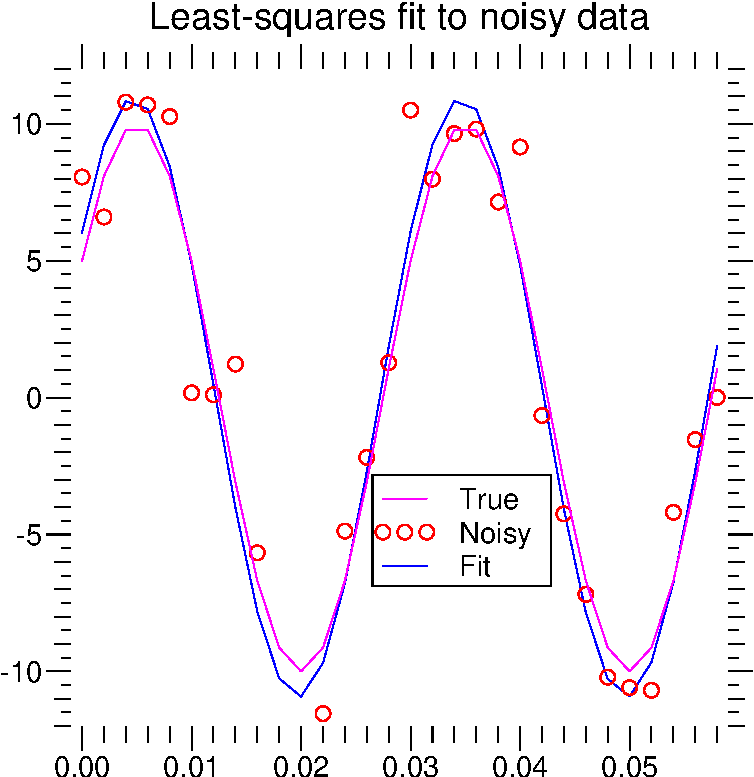
\includegraphics{leastsqfit.epsi}} \par}


\caption{\label{fig:least_squares_fit}Least-square fitting to noisy data
using \textbf{scipy.optimize.leastsq}}
\end{figure}



\subsection{Bounded minimization (optimize.fminbound)}

Thus far all of the minimization routines described have been unconstrained
minimization routines. Very often, however, there are constraints
that can be placed on the solution space before minimization occurs.
The \textbf{fminbound} function is an example of a constrained minimization
procedure that provides a rudimentary interval constraint for scalar
functions (functions which take a scalar input and return a scalar
output). The interval constraint allows the minimization to occur
only between two fixed endpoints.

For example, to find the minimum of \( J_{1}\left( x\right)  \) near
\( x=5 \), \textbf{fminbound} can be called using the interval \( \left[ 4,7\right]  \)
as a constraint. The result is \( x_{\textrm{min}}=5.3314 \):

\verbatiminput{example5.8}


\subsection{Root finding (optimize.fsolve)}

To find the roots of a polynomial, the command \textbf{roots} from
Numeric Python is useful (this is also available as \textbf{roots}).
To find a root of a set of non-linear equations, the command \textbf{optimize.fsolve}
is needed. For example, the following example finds the roots of the
single-variable transcendental equation\[
x+2\cos \left( x\right) =0,\]
 and the set of non-linear equations\begin{eqnarray*}
x_{0}\cos \left( x_{1}\right)  & = & 4,\\
x_{0}x_{1}-x_{1} & = & 5.
\end{eqnarray*}
 The results are \( x=-1.0299 \) and \( x_{0}=6.5041,\, x_{1}=0.9084 \).

\verbatiminput{example5.9}


\section{Interpolation (interpolate)}

There are two general interpolation facilities available in SciPy.
The first facility is an interpolation class which performs linear
1-dimensional interpolation. The second facility is based on the FORTRAN
library FITPACK and provides functions for 1- and 2-dimensional (smoothed)
cubic-spline interpolation. 


\subsection{Linear 1-d interpolation (interpolate.linear\_1d)}

The linear\_1d class in scipy.interpolate is a convenient method to
create a function based on fixed data points which can be evaluated
anywhere within the domain defined by the given data using linear
interpolation. An instance of this class is created by passing the
1-d vectors comprising the data. The instance of this class defines
a \emph{\_\_call\_\_} method and can therefore by treated like a function
which interpolates between known data values to obtain unknown values
(it even has a docstring for help). Behavior at the boundary can be
specified at instantiation time. The following example demonstrates
it's use. 

\verbatiminput{example6.1}Figure shows the result: 
\begin{figure}
{\centering \resizebox*{0.5\textwidth}{!}{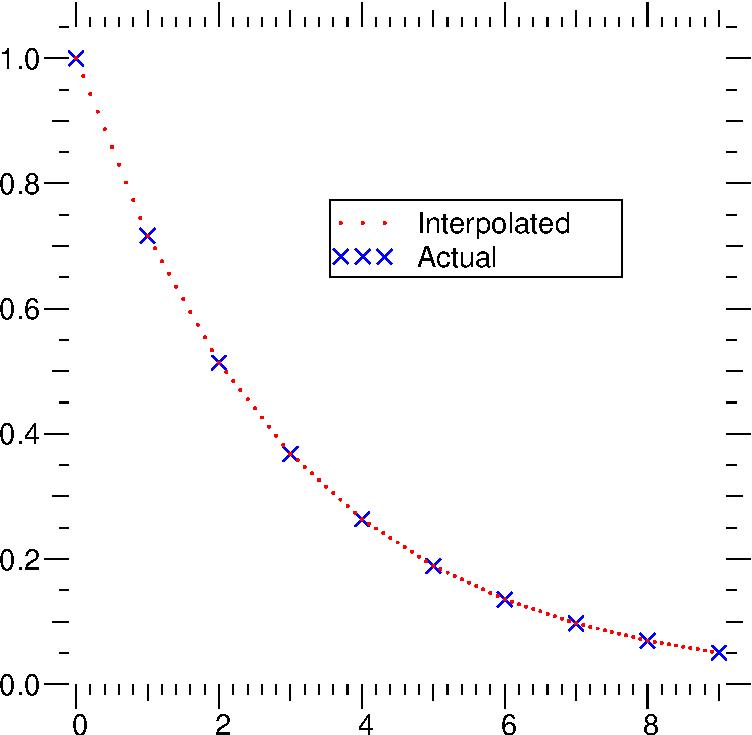
\includegraphics{inter_1d.epsi}} \par}


\caption{\label{fig:inter_1d}One-dimensional interpolation using the class
\textbf{interpolate.linear\_1d.}}
\end{figure}



\subsection{Spline interpolation in 1-d (interpolate.splXXX)}

Spline interpolation requires two essential steps: (1) a spline representation
of the curve is computed, and (2) the spline is evaluated at the desired
points. In order to find the spline representation, there are two
different was to represent a curve and obtain (smoothing) spline coefficients:
directly and parametrically. The direct method finds the spline representation
of a curve in a two-dimensional plane using the function \textbf{interpolate.splrep.}
The first two arguments are the only ones required, and these provide
the \( x \) and \( y \) components of the curve. The normal output
is a 3-tuple, \( \left( t,c,k\right)  \), containing the knot-points,
\( t \), the coefficients \( c \) and the order \( k \) of the
spline. The default spline order is cubic, but this can be changed
with the input keyword, \emph{k.}

For curves in \( N \)-dimensional space the function \textbf{interpolate.splprep}
allows defining the curve parametrically. For this function only 1
input argument is required. This input is a list of \( N \)-arrays
representing the curve in \( N \)-dimensional space. The length of
each array is the number of curve points, and each array provides
one component of the \( N \)-dimensional data point. The parameter
variable is given with the keword argument, \emph{u,} which defaults
to an equally-spaced monotonic sequence between \( 0 \) and \( 1 \).
The default output consists of two objects: a 3-tuple, \( \left( t,c,k\right)  \),
containing the spline representation and the parameter variable \( u. \) 

The keyword argument, \emph{s}, is used to specify the amount of smoothing
to perform during the spline fit. The default value of \( s \) is
\( s=m-\sqrt{2m} \) where \( m \) is the number of data-points being
fit. Therefore, \textbf{if no smoothing is desired a value of \( \mathbf{s}=0 \)
should be passed to the routines. }

Once the spline representation of the data has been determined, functions
are available for evaluating the spline (\textbf{interpolate.splev)}
and its derivatives (\textbf{interpolate.splev, interpolate.splade})
at any point and the integral of the spline between any two points
(\textbf{interpolate.splint)}. In addition, for cubic splines (\( k=3 \))
with 8 or more knots, the roots of the spline can be estimated (\textbf{interpolate.sproot)}.
These functions are demonstrated in the example that follows (see
also Figure \ref{fig:spline-1d}).


\begin{figure}
{\centering \subfigure[Cubic-spline (splrep)]{\resizebox*{0.45\textwidth}{!}{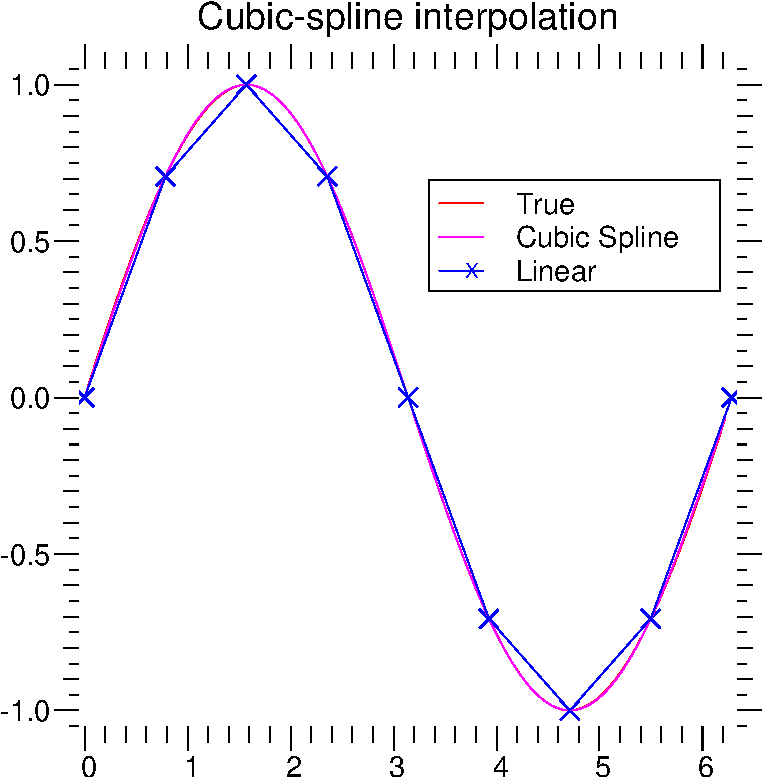
\includegraphics{interp_cubic.epsi}}} \subfigure[Derivative of spline (splev)]{\resizebox*{0.45\textwidth}{!}{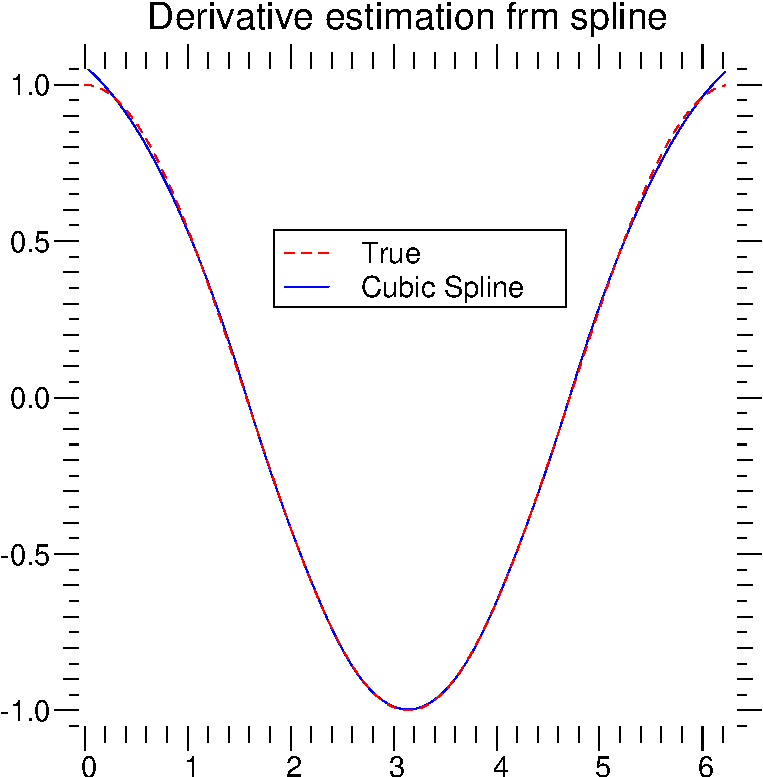
\includegraphics{interp_cubic_der.epsi}}} \par}

{\centering \subfigure[Integral of spline (splint)]{\resizebox*{0.45\textwidth}{!}{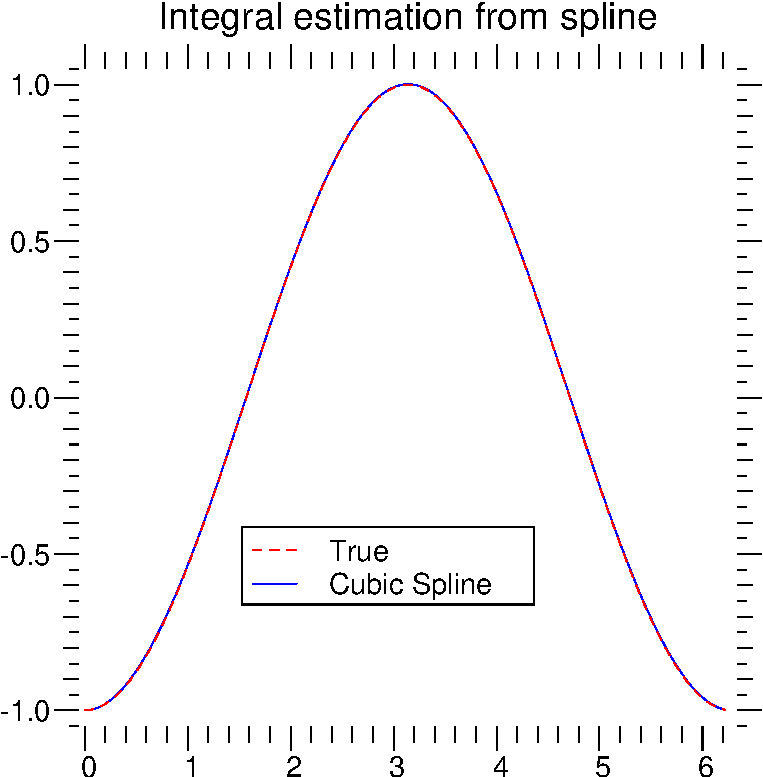
\includegraphics{interp_cubic_int.epsi}}} \subfigure[Spline of parametric curve (splprep)]{\resizebox*{0.45\textwidth}{!}{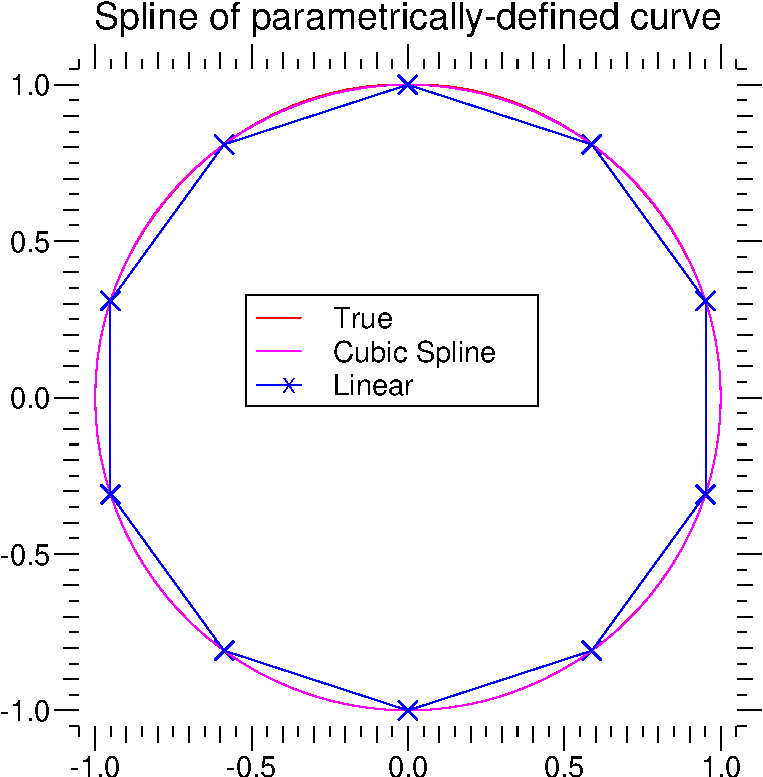
\includegraphics{interp_cubic_param.epsi}}} \par}


\caption{\label{fig:spline-1d}Examples of using cubic-spline interpolation.}
\end{figure}


\verbatiminput{example6.2}


\subsection{Two-dimensionsal spline representation (interpolate.bisplrep)}

For (smooth) spline-fitting to a two dimensional surface, the function
\textbf{interpolate.bisplrep} is available. This function takes as
required inputs the \textbf{1-D} arrays \emph{x, y,} and \emph{z}
which represent points on the surface \( z=f\left( x,y\right) . \)
The default output is a list \( \left[ tx,ty,c,kx,ky\right]  \) whose
entries represent respectively, the components of the knot positions,
the coefficients of the spline, and the order of the spline in each
coordinate. It is convenient to hold this list in a single object,
\emph{tck,} so that it can be passed easily to the function \textbf{interpolate.bisplev.}
The keyword, \emph{s}, \emph{}can be used to change the amount of
smoothing performed on the data while determining the appropriate
spline. The default value is \( s=m-\sqrt{2m} \) where \( m \) is
the number of data points in the \emph{x, y,} and \emph{z} vectors.
As a result, if no smoothing is desired, then \( s=0 \) should be
passed to \textbf{interpolate.bisplrep.}

To evaluate the two-dimensional spline and it's partial derivatives
(up to the order of the spline), the function \textbf{interpolate.bisplev}
is required. This function takes as the first two arguments \textbf{two
1-D arrays} whose cross-product specifies the domain over which to
evaluate the spline. The third argument is the \emph{tck} list returned
from \textbf{interpolate.bisplrep.} If desired, the fourth and fifth
arguments provide the orders of the partial derivative in the \( x \)
and \( y \) direction respectively. 

It is important to note that two dimensional interpolation should
not be used to find the spline representation of images. The algorithm
used is not amenable to large numbers of input points. The signal
processing toolbox contains (soon) more appropriate algorithms for
finding the spline representation of an image. The two dimensional
interpolation commands are intended for use when interpolating a two
dimensional function as shown in the example that follows (See also
Figure \ref{fig:2d_interp}). This example uses the \textbf{grid}
command in SciPy which is useful for defining a {}``mesh-grid{}''
in many dimensions. The number of output arguments and the number
of dimensions of each argument is determined by the number of indexing
objects passed in \textbf{grid}[]. \verbatiminput{example6.3}

\vspace{0.3cm}
{
\begin{figure}
{\centering \resizebox*{0.45\textwidth}{!}{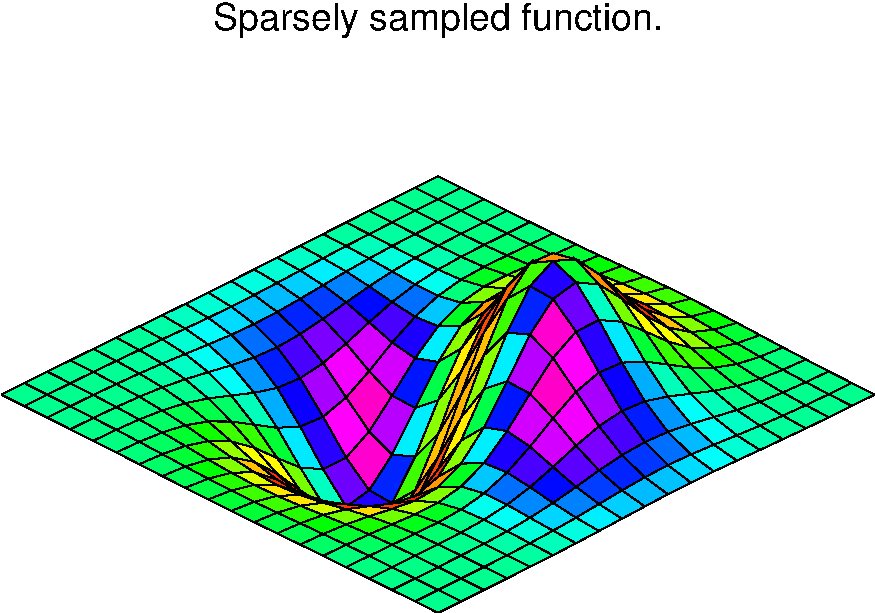
\includegraphics{2d_func.epsi}} ~~\resizebox*{0.45\textwidth}{!}{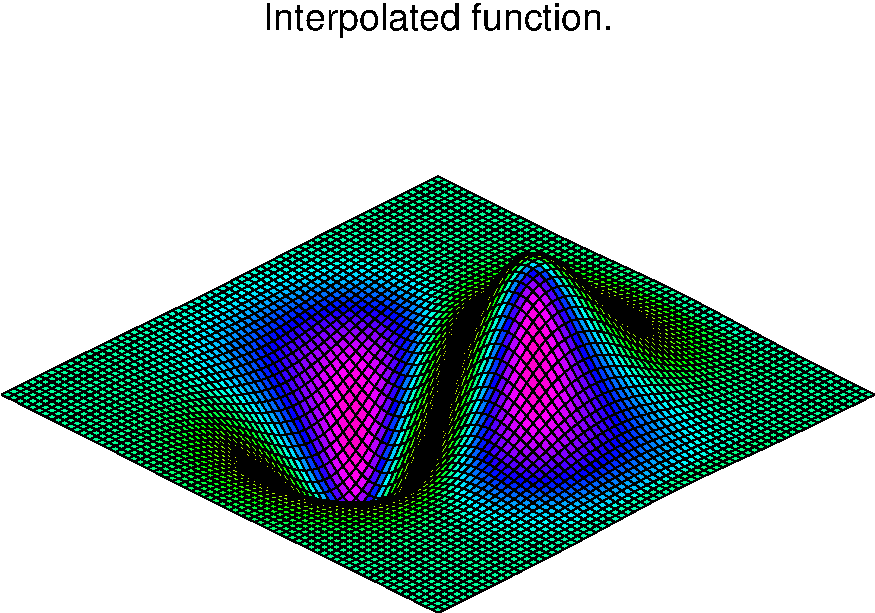
\includegraphics{2d_interp.epsi}} \par}


\caption{\label{fig:2d_interp}Example of two-dimensional spline interpolation.}
\end{figure}
\par}
\vspace{0.3cm}


\section{Signal Processing}

The signal processing toolbox currently contains some filtering functions
and a limited set of filter design tools. This box should steadly 
\end{document}
